\documentclass[conference]{IEEEtran}
\IEEEoverridecommandlockouts

\usepackage{cite}
\usepackage{amsmath,amssymb,amsfonts}
\usepackage{algorithmic}
\usepackage{graphicx}
\usepackage{textcomp}
\usepackage{xcolor}
\usepackage{booktabs}
\usepackage{multirow}
\usepackage{pifont}   % for \ding{51} checkmark
\usepackage{tikz}
\usetikzlibrary{arrows.meta, positioning}
\usepackage[colorlinks=true,
            linkcolor=black,
            citecolor=black,
            urlcolor=blue,
            pdftitle={ModalIn: Decentralized P2P Micro-Lending},
            pdfauthor={Zebua, Katoroy, Sitio}]{hyperref}

\newcommand{\cmark}{\ding{51}}  % checkmark symbol

\def\BibTeX{{\rm B\kern-.05em{\sc i\kern-.025em b}\kern-.08em
    T\kern-.1667em\lower.7ex\hbox{E}\kern-.125emX}}

% ---------------------------------------------------------------
% TikZ styles
% ---------------------------------------------------------------
\tikzset{
  fbox/.style={rectangle, draw, fill=blue!12, rounded corners=2pt,
               align=center, minimum height=1.8em, minimum width=3.5cm,
               font=\scriptsize},
  cbox/.style={rectangle, draw, fill=orange!18, rounded corners=2pt,
               align=center, minimum height=1.8em,
               font=\scriptsize},
  sbox/.style={rectangle, draw=gray!60, fill=gray!8, rounded corners=2pt,
               align=center, minimum height=1.8em, minimum width=1.6cm,
               font=\scriptsize},
  marr/.style={-{Stealth[length=3.5pt]}, semithick}
}

\begin{document}

% ---------------------------------------------------------------
% TITLE
% ---------------------------------------------------------------
\title{ModalIn: Decentralized P2P Micro-Lending with On-Chain Reputation
Using Soulbound Tokens and Social Trust Primitives for Indonesian MSMEs}

% ---------------------------------------------------------------
% AUTHORS  (three equal columns)
% ---------------------------------------------------------------
\author{
  \IEEEauthorblockN{Abednego Zebua}
  \IEEEauthorblockA{
    \textit{Computer Engineering Program}\\
    \textit{Universitas Indonesia}\\
    Depok, Indonesia\\
    abednego.zebua@ui.ac.id}
  \and
  \IEEEauthorblockN{Calvin Wirathama Katoroy}
  \IEEEauthorblockA{
    \textit{Computer Engineering Program}\\
    \textit{Universitas Indonesia}\\
    Depok, Indonesia\\
    calvin.wirathama@ui.ac.id}
  \and
  \IEEEauthorblockN{Wilman Saragih Sitio}
  \IEEEauthorblockA{
    \textit{Computer Engineering Program}\\
    \textit{Universitas Indonesia}\\
    Depok, Indonesia\\
    wilman.saragih@ui.ac.id}
}

\maketitle

% ---------------------------------------------------------------
% ABSTRACT
% ---------------------------------------------------------------
\begin{abstract}
Indonesia's 64 million micro, small, and medium enterprises (MSMEs) contribute
61\% of national GDP yet face a credit gap exceeding Rp~2,800~trillion annually.
This gap persists because conventional lenders require documented repayment
histories and physical collateral that most MSME operators cannot provide.
Existing decentralized finance (DeFi) platforms fail this population equally,
as they impose overcollateralization requirements in crypto assets that remain
inaccessible to unbanked borrowers.

We present ModalIn, an Ethereum-based peer-to-peer micro-lending decentralized
application (DApp) that replaces physical collateral with a triple-layer
on-chain reputation system. ModalIn issues each borrower a non-transferable
Soulbound Token (SBT) as a persistent credit identity, organizes borrowers
into tiered Credit Guilds formalizing Indonesia's collective accountability
culture, and enables ETH-staked peer vouching as social guarantee.
A composite reputation score weighted 70\% payment history and 30\% peer
vouch drives an algorithmic annual percentage rate (APR) model bounded
between 6\% and 36\% in alignment with Indonesian Financial Services Authority
(OJK) reference bounds. Validated by 29 passing automated test scenarios
across six Solidity smart contracts, the system demonstrates up to a 65\%
reduction in borrowing cost for high-reputation borrowers compared to unscored
entrants, and a minimum threefold improvement over typical informal moneylender
rates.
\end{abstract}

\begin{IEEEkeywords}
blockchain, credit scoring, decentralized finance, micro-lending, soulbound token
\end{IEEEkeywords}

% ---------------------------------------------------------------
% I. INTRODUCTION
% ---------------------------------------------------------------
\section{Introduction}

Micro, small, and medium enterprises (MSMEs) form the backbone of Indonesia's
economy. With over 64~million units, they contribute approximately 61\% of
national gross domestic product and absorb 97\% of the domestic
workforce~\cite{b4}. Despite this economic significance, more than 40\% of
Indonesian MSMEs lack access to formal banking credit, creating a financing gap
estimated at over Rp~2,800~trillion per year~\cite{b4,b15}. Global evidence
confirms that this structural exclusion is especially acute in archipelagic
and developing economies where rural enterprises have limited contact with
formal financial institutions~\cite{b16,b17}. The root causes are structural:
conventional credit scoring systems require documented repayment histories and
physical assets as collateral, prerequisites that most informal-sector MSME
operators cannot meet~\cite{b3}.

MSME operators who lack formal credit access turn to informal moneylenders
(\textit{rentenir}), whose annualized interest rates commonly reach
20\%--60\%~\cite{b9}. This exploitative cost of capital prevents accumulation
of operating surplus, which in turn prevents the formation of credit history
needed to qualify for cheaper formal loans. The resulting debt trap imposes a
structural ceiling on enterprise growth, disproportionately affecting
women-owned and rural businesses that constitute the majority of the MSME
sector~\cite{b17}.

Blockchain technology~\cite{b11,b18} offers a structural solution by resolving
information asymmetry between lenders and borrowers without a trusted
intermediary~\cite{b4}. The immutability of on-chain records ensures that
repayment history cannot be manipulated, providing lenders with mathematical
certainty. The Soulbound Token (SBT), a non-transferable, wallet-bound digital
artifact representing commitments and credentials~\cite{b1,b2}, enables a
persistent, unforgeable credit identity that follows a borrower across all
transactions on the network. Smart contracts~\cite{b19} self-execute lending
terms when predefined conditions are met, eliminating the processing delays
and costs of human underwriting.

Critically, Indonesian informal credit culture already embeds the primitives
needed for reputation-based lending. The \textit{arisan} (rotating savings
group), \textit{koperasi} (cooperative), and \textit{gotong royong} (mutual
aid) traditions demonstrate that collective accountability and social guarantee
are culturally validated mechanisms for reducing default risk. What has been
missing is infrastructure that encodes these social trust mechanisms into
verifiable, immutable on-chain data.

We present ModalIn, a decentralized P2P micro-lending DApp that translates
these cultural trust primitives into smart contract logic on the Ethereum
Virtual Machine (EVM). The contributions of this paper are:

\begin{enumerate}
\item A triple-layer on-chain reputation model combining payment history
(70\%), ETH-staked peer vouching (30\%), and an extensible oracle attestation
slot (reserved for future integration via the Ethereum Attestation
Service~\cite{b6}) into a composite credit score on a 0--1000 scale, with
formal weight assignment and a time-based reputation decay mechanism
(Section~III-B).

\item An algorithmic interest rate model computing APR directly from on-chain
reputation and group tier, with OJK-referenced bounds (6\%--36\%), eliminating
manual underwriting (Section~III-A).

\item A Credit Guild mechanism (Bronze/Silver/Gold tier) formalizing
\textit{gotong royong} collective accountability as a smart contract primitive
with group-level score propagation (Section~III-D).

\item A full working DApp comprising six Solidity contracts (Hardhat~3.1.12,
OpenZeppelin~v5.6), a React~19 frontend with ethers.js~v6 integration,
validated by 29 automated test scenarios on a local Hardhat development node
with Ethereum Sepolia testnet deployment support (Sections~IV--VI).
\end{enumerate}

The remainder of this paper is organized as follows.
Section~II surveys related work on DeFi lending protocols, group lending
models, blockchain-based SME finance, and on-chain reputation systems.
Section~III formalizes the proposed reputation scoring and interest rate
models. Section~IV describes the system architecture and smart contract
design. Section~V covers implementation details and key engineering decisions.
Section~VI reports testing, evaluation, and a comparative discussion.
Section~VII concludes with a discussion of future work directions and
open challenges.

% ---------------------------------------------------------------
% II. RELATED WORK
% ---------------------------------------------------------------
\section{Related Work}

\subsection{Overcollateralized DeFi Lending}

The majority of production DeFi lending protocols operate on an
overcollateralized model~\cite{b20}. Dominant protocols such as Aave and
Compound require borrowers to lock crypto assets worth 120\%--150\% of the
loan value~\cite{b7}. While this protects lenders against price volatility,
it is fundamentally inaccessible to MSMEs who hold no crypto assets.
Yan~et~al.~\cite{b7} analyzed blockchain as a solution for P2P lending
fraud, concluding that on-chain immutability addresses the core trust problem
but the work offered no mechanism for unsecured lending.
Goldfinch~\cite{b14} partially addresses collateral requirements
by introducing off-chain trust anchors, but still relies on institutional
backers rather than individual on-chain reputation. ModalIn departs from this
paradigm entirely: no crypto collateral is required, and on-chain reputation
is the sole substitute for collateral.

\subsection{Traditional Group Lending}

Group-lending microfinance models such as the Grameen Bank~\cite{b13}
demonstrate that collective accountability and peer pressure reduce default
rates significantly in microcredit populations with no physical collateral.
Bambico~et~al.~\cite{b21} find that behavioral and payment-pattern features
are the strongest predictors of loan repayment outcomes, validating the
primacy of on-chain repayment records over static creditworthiness proxies.
However, Grameen's model is manual, centralized, and non-auditable at global
scale. ModalIn encodes the same social accountability mechanism (collective
responsibility, tiered trust, and social guarantee) as immutable smart
contract logic, preserving the behavioral incentive while removing the
operational overhead.

\subsection{Blockchain for SME Finance}

Kumar~et~al.~\cite{b4} conducted a systematic review of blockchain-based SME
finance and found strong evidence that distributed ledgers reduce information
asymmetry and transaction costs, but their work remains a literature review
without a system architecture. Hoque~et~al.~\cite{b3} investigated blockchain-based microcredit platforms
in developing countries and identified credible on-chain financial profiles
as the key opportunity for lending inclusion.
Yan~et~al.~\cite{b7} analyzed blockchain as a solution for P2P lending fraud,
concluding that immutability and smart contracts address herding and collusion
but leave credit scoring unresolved. Nanayakkara~et~al.~\cite{b5} proposed swarm
learning for P2P credit scoring, but their approach relies on off-chain
machine learning rather than on-chain identity primitives, which means credit
scores remain opaque and centrally controlled.

\subsection{On-Chain Reputation and Soulbound Tokens}

Weyl, Ohlhaver, and Buterin~\cite{b1} introduced Decentralized Society
(DeSoc) and SBTs as non-transferable tokens encoding social relationships
and credentials. EIP-5114~\cite{b12} standardizes the Soulbound Badge
interface. Pinna~et~al.~\cite{b22} survey SBT applications across digital identity,
governance, and reputation contexts, observing that non-transferability and
wallet-binding make SBTs uniquely suited as credible on-chain reputation
carriers; ModalIn operationalizes these properties specifically for credit
scoring with a weighted multi-dimensional formula.
Table~\ref{tab:related} positions ModalIn against the most closely related
systems.

\begin{table}[t]
\caption{Comparison of Related Systems}
\label{tab:related}
\centering
{\small
\setlength{\tabcolsep}{3pt}
\begin{tabular}{p{1.6cm}p{1.9cm}p{2.3cm}p{1.2cm}}
\toprule
\textbf{System} & \textbf{Mechanism} & \textbf{Key Limitation} & \textbf{Collat.} \\
\midrule
Aave / Compound & Overcollateral   & Excludes unbanked      & Crypto \\
Grameen Bank  & Group lending    & Manual, centralized    & Social \\
Goldfinch     & Off-chain trust  & Institutional backers  & Off-chain \\
Kumar et al.  & Review only      & No architecture        & N/A \\
\textbf{ModalIn} & \textbf{SBT + Guild}\newline\textbf{+ Vouch} & \textbf{ETH-only amounts} & \textbf{Reputation} \\
\bottomrule
\end{tabular}}
\end{table}

% ---------------------------------------------------------------
% III. PROPOSED METHOD
% ---------------------------------------------------------------
\section{Proposed Method}

\subsection{Problem Formalization}

Given a borrower $b$ with no prior formal credit record, we seek to compute a
verifiable trust score $S(b) \in [0, 1000]$ derived solely from on-chain
behavior, and use it to determine a fair lending APR in accordance with
OJK-referenced regulatory bounds~\cite{b23}:
%
\begin{equation}
\text{APR}(b) = \text{BaseRate} + \text{GroupPremium}(b) - \text{RepDiscount}(b)
\label{eq:apr}
\end{equation}
%
where all terms are in basis points (1~bps $= 0.01\%$), and APR is clamped to
$[\text{APR}_\text{min},\, \text{APR}_\text{max}] = [600,\, 3600]$~bps,
corresponding to 6\%--36\% annually.

\subsection{Triple-Layer Reputation Model}

The composite credit score aggregates three orthogonal trust signals:
%
\begin{equation}
S(b) = \frac{w_p \cdot P(b) + w_v \cdot V(b) + w_a \cdot A(b)}{100}
\label{eq:score}
\end{equation}
%
where $P(b) \in [0, 1000]$ is the \textit{payment score} computed as $10r$
with $r = (\text{loans repaid} / \text{loans taken}) \times 100$; $V(b)
\in [0, 1000]$ is the \textit{vouch score} from ETH-staked peer guarantees
computed by \texttt{VouchRegistry}; $A(b) \in [0, 1000]$ is the
\textit{attestation score} from an authorized oracle (e.g., e-commerce
transaction data); and deployed weights $w_p = 70$, $w_v = 30$, $w_a = 0$
sum to 100 ($w_a = 0$ reflects oracle attestation reserved for future
integration via the Ethereum Attestation Service~\cite{b6}).

The weight assignment reflects a hierarchy of manipulation resistance grounded
in empirical findings from the microfinance and P2P credit-scoring literature.
Bambico~et~al.~\cite{b21} find that behavioral and payment-pattern features
are the strongest predictors of loan repayment outcomes in microfinance
populations; Nanayakkara~et~al.~\cite{b5} similarly identify transaction
history as the highest-weighted feature in P2P lending credit-scoring models.
Payment history ($w_p = 70$) is therefore weighted highest: it is fully
on-chain, hardest to forge, and requires a borrower to have completed actual
loan repayments, making it the most direct and tamper-resistant behavioral
signal available. Peer vouching ($w_v = 30$) requires real ETH at economic
risk, imposing a tangible cost on misrepresentation; however, coordinated
ring-vouching among colluding peers remains a theoretical attack vector,
warranting a lower weight than raw repayment history. Attestation ($w_a = 0$)
carries oracle centralization risk in its current single-address form, so
this component is excluded from the live deployment until a decentralized
attestation infrastructure is available~\cite{b6}. These three distinct
signals are necessary because no single on-chain observable is sufficient:
payment history alone ignores social context, and vouching alone is vulnerable
to collusion without the behavioral anchor that repayment history provides.

\subsection{Reputation Decay}

To prevent stale high scores from being exploited, a time-based decay applies
a penalty of 10~points per 180-day period of inactivity:
%
\begin{equation}
S_\text{final}(b) = \max\!\left(0,\; S(b) - 10
  \left\lfloor \frac{t_\text{now} - t_\text{last}}{T_\text{decay}}
  \right\rfloor \right)
\label{eq:decay}
\end{equation}
%
where $T_\text{decay} = 180$~days and $t_\text{last}$ is the timestamp of the
last on-chain update stored in the borrower's SBT profile.

\subsection{Social Trust Mapping}

A central design insight of ModalIn is the direct mapping of Indonesian social
trust practices to on-chain primitives, as shown in Table~\ref{tab:mapping}.

The \textit{arisan} and \textit{koperasi} traditions organize lending around
group membership and collective reputation. This is mirrored by the Credit
Guild system, which groups borrowers into scored cohorts where default by
any member propagates a penalty to the group average score, creating the same
mutual monitoring incentive observed in cooperative finance. The
\textit{jaminan} (guarantee) custom, under which a community member stands
surety for a borrower, is formalized as ETH-staked peer vouching: vouchers
commit economic value on-chain, and stake is slashed algorithmically upon
borrower default, eliminating the enforcement ambiguity of informal
guarantees. The \textit{gotong royong} ethic of collective responsibility is
thus encoded not as a cultural appeal but as a self-enforcing economic
constraint: defection becomes more costly than cooperation.
Pinna~et~al.~\cite{b22} observe that the credibility of on-chain reputation
derives from its non-transferable, wallet-bound nature; both properties
are reinforced in ModalIn through the soulbound identity and the
ETH-staked vouching mechanism.

\begin{table}[t]
\caption{Indonesian Social Trust to Smart Contract Mapping}
\label{tab:mapping}
\centering
\begin{tabular}{p{1.9cm}p{2.0cm}p{2.0cm}}
\toprule
\textbf{Indonesian Tradition} & \textbf{ModalIn Mechanism} & \textbf{Contract} \\
\midrule
Credit bureau / bank history  & Payment score via SBT & \texttt{SoulboundToken} \\
\textit{Koperasi / Arisan}    & Credit Guild (Bronze/Silver/Gold) & \texttt{GuildSBT} \\
\textit{Jaminan} / guarantee  & Peer vouch + ETH slash & \texttt{VouchRegistry} \\
Merchant sales data           & Attestation oracle     & \texttt{ReputationEngine} \\
Loan escrow                   & P2P lifecycle          & \texttt{LoanEscrow} \\
\bottomrule
\end{tabular}
\end{table}

% ---------------------------------------------------------------
% IV. SYSTEM DESIGN
% ---------------------------------------------------------------
\section{System Design}

\subsection{Architecture Overview}

ModalIn adopts a strict separation-of-concerns architecture across two layers,
as shown in Fig.~\ref{fig:arch}. The \textit{Frontend Layer} is a React~19
web application that communicates through ethers.js~v6 and a MetaMask wallet
extension. All state-changing interactions are submitted as cryptographically
signed transactions; no centralized database stores any loan or reputation
state. The \textit{Blockchain Protocol Layer} consists of six Solidity
contracts with a defined dependency hierarchy: \texttt{LoanEscrow} is the
primary orchestrator, delegating APR computation to
\texttt{InterestRateModel} and reputation updates to
\texttt{ReputationEngine}, which reads from and writes to
\texttt{SoulboundToken}, \texttt{GuildSBT}, and \texttt{VouchRegistry}.

\begin{figure}[t]
\centering
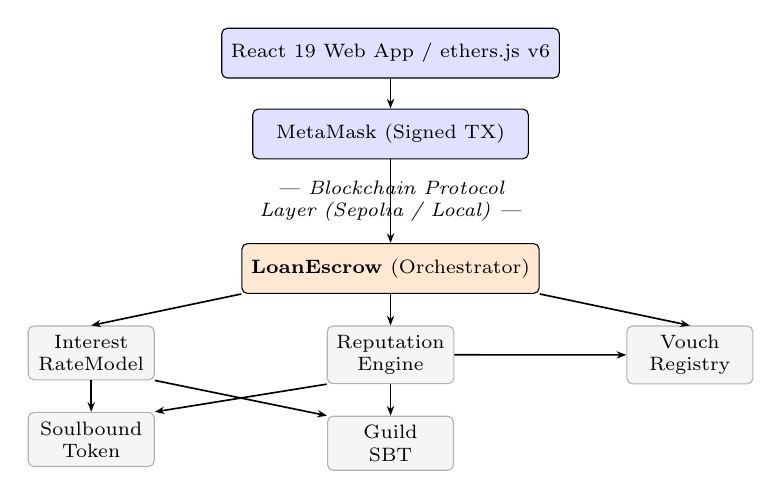
\begin{tikzpicture}[node distance=0.38cm and 0.4cm]
  %% -- Frontend layer --
  \node[fbox] (react) {React~19 Web App / ethers.js v6};
  \node[fbox, below=of react] (mm) {MetaMask (Signed TX)};

  %% -- Layer separator label --
  \node[font=\scriptsize\itshape, below=0.15cm of mm,
        text width=3.5cm, align=center] (sep)
    {--- Blockchain Protocol Layer (Sepolia / Local) ---};

  %% -- Main orchestrator --
  \node[cbox, minimum width=3.5cm, below=0.15cm of sep] (escrow)
    {\textbf{LoanEscrow} (Orchestrator)};

  %% -- Second tier --
  \node[sbox, below left=0.4cm and 1.1cm of escrow]  (irm)
    {Interest\\RateModel};
  \node[sbox, below=0.4cm of escrow]                  (re)
    {Reputation\\Engine};
  \node[sbox, below right=0.4cm and 1.1cm of escrow] (vouch)
    {Vouch\\Registry};

  %% -- Third tier --
  \node[sbox, below=0.4cm of irm]   (sbt)   {Soulbound\\Token};
  \node[sbox, below=0.4cm of re]    (guild) {Guild\\SBT};

  %% -- Arrows: frontend --
  \draw[marr] (react)  -- (mm);
  \draw[marr] (mm)     -- (escrow);

  %% -- Arrows: orchestrator to second tier --
  \draw[marr] (escrow.south west) -- (irm.north);
  \draw[marr] (escrow.south)      -- (re.north);
  \draw[marr] (escrow.south east) -- (vouch.north);

  %% -- Arrows: second to third tier --
  \draw[marr] (irm.south)     -- (sbt.north);
  \draw[marr] (irm.south east) -- (guild.north west);
  \draw[marr] (re.south)      -- (guild.north);
  \draw[marr] (re.south west) -- (sbt.north east);
  \draw[marr] (re.east)       -- (vouch.west);
\end{tikzpicture}
\caption{ModalIn two-layer architecture. The frontend communicates exclusively
through signed transactions; all loan and reputation state is stored on-chain.}
\label{fig:arch}
\end{figure}

\subsection{Smart Contract Design}

Table~\ref{tab:contracts} summarizes the six contracts and their
responsibilities. The \texttt{SoulboundToken} stores each borrower's
\texttt{CreditProfile} struct (encompassing loan counts, cumulative amounts,
reputation score, and last-updated timestamp) and starts new borrowers at a
neutral score of 500. The \texttt{GuildSBT} assigns tier based on collective
average score: Bronze ($S < 650$), Silver ($650 \leq S < 800$), Gold
($S \geq 800$). The \texttt{VouchRegistry} records ETH-staked peer guarantees
and slashes stakes proportionally upon borrower default.

\begin{table}[t]
\caption{Smart Contract Summary}
\label{tab:contracts}
\centering
\begin{tabular}{p{1.9cm}p{4.7cm}}
\toprule
\textbf{Contract} & \textbf{Key Responsibility} \\
\midrule
\texttt{Soulbound}\newline\texttt{Token}
  & Non-transferable ERC-5114-inspired credit identity; stores \texttt{CreditProfile}; starting score 500; all token transfers permanently revert. \\[2pt]
\texttt{GuildSBT}
  & Credit group (2--10 members); tier Bronze/Silver/Gold from collective score; tier updates on score recalculation. \\[2pt]
\texttt{VouchRegistry}
  & ETH-staked peer vouches; stake-weighted vouch score; slashes on default. \\[2pt]
\texttt{Reputation}\newline\texttt{Engine}
  & Aggregates $S(b)$ per~\eqref{eq:score}; applies decay per~\eqref{eq:decay}; propagates to guild average. \\[2pt]
\texttt{InterestRate}\newline\texttt{Model}
  & APR per~\eqref{eq:apr}: Bronze +800~bps, Silver +400~bps, Gold +0~bps; reputation discount up to $-600$~bps. \\[2pt]
\texttt{LoanEscrow}
  & Loan states: Requested $\to$ Active $\to$ Repaid/Defaulted; holds ETH in escrow; triggers reputation update on resolution. \\
\bottomrule
\end{tabular}
\end{table}

\subsection{Access Control and Security Design}

Sensitive state-writing operations are protected by an authorized-callers
whitelist pattern rather than role-based access control, keeping gas overhead
low while preventing unauthorized score manipulation. All Ether-moving
operations use OpenZeppelin's reentrancy guard~\cite{b22_oz}. The
\texttt{LoanEscrow} contract additionally follows the Checks-Effects-Interactions
(CEI) pattern: all state updates precede external Ether transfers, eliminating
reentrancy vectors by design.

% ---------------------------------------------------------------
% V. IMPLEMENTATION
% ---------------------------------------------------------------
\section{Implementation}

\subsection{Technology Stack}

Table~\ref{tab:stack} lists the exact component versions used in ModalIn.

\begin{table}[t]
\caption{Technology Stack}
\label{tab:stack}
\centering
\begin{tabular}{lll}
\toprule
\textbf{Component} & \textbf{Version} & \textbf{Role} \\
\midrule
Solidity          & 0.8.20   & Smart contract language \\
Hardhat           & 3.1.12   & EVM dev environment \\
OpenZeppelin      & v5.6.1   & Ownable, ReentrancyGuard \\
ethers.js         & v6.16.0  & Frontend--contract bridge \\
React             & 19       & Frontend framework \\
TypeScript        & v5.8.2   & Frontend type safety \\
Vite              & v6.2.0   & Build toolchain \\
TailwindCSS       & v4.1.14  & UI styling \\
Mocha / Chai      & 11.x / 6.x & Test runner / assertions \\
Node.js           & v24.11.1 & Runtime environment \\
\bottomrule
\end{tabular}
\end{table}

\subsection{Deployment Strategy}

Two deployment environments are supported. For local development,
the Hardhat local node instantiates a simulated EVM (Chain~ID~31337) with
controllable block timestamps, enabling testing of deadline and decay
scenarios. The deploy script deploys all six contracts in dependency order and
injects their addresses into
\texttt{modalin-frontend/src/abis/contract-addresses.json}, making the
frontend environment-agnostic. For public validation, contracts are deployable
to the \textit{Ethereum Sepolia testnet} (Proof of Stake) via the included
\texttt{deploy:sepolia} script, demonstrating viability with real consensus
and block finality.

\subsection{Key Implementation Decisions}

\textit{Basis-point APR arithmetic.} Solidity does not support
floating-point~\cite{b8,b24}. All rates are stored in integer basis points
and interest is computed as:
\[
  \text{interest} =
  \frac{\text{principal} \times \text{APR(bps)} \times \text{days}}
       {365 \times 10000}
\]

\textit{Self-registration.} Any wallet can issue its own SBT on first
connection, eliminating admin-gated onboarding and reducing entry friction for
MSME users unfamiliar with blockchain-based identity systems.

\textit{Guild size cap.} Membership is capped at 10 per group to bound the
iteration in the collective score recalculation loop, preventing out-of-gas
exceptions on the EVM.

\textit{Custom Solidity errors.} All revert conditions use typed error
declarations instead of string messages, reducing deployment and call gas
costs.

% ---------------------------------------------------------------
% VI. TESTING AND EVALUATION
% ---------------------------------------------------------------
\section{Testing and Evaluation}

\subsection{Test Suite and Hardware Environment}

ModalIn employs a three-level testing strategy: (1)~unit testing, with each
contract function tested in isolation; (2)~integration testing of
cross-contract interactions (e.g., the loan escrow invoking the reputation
engine on repayment); and (3)~manual UI testing consisting of end-to-end
simulation via the frontend and MetaMask to validate the borrower and lender
user journeys.
The automated suite uses Hardhat's time-manipulation RPC call to advance
block timestamps, enabling deadline and decay scenarios without waiting for
real time to elapse.

All tests were executed on a development workstation running Windows~11
Home (64-bit) with an Intel Core~i7 processor and 16~GB DDR4~RAM.
The Hardhat local node operated on Node.js~v24.11.1 under Chain~ID~31337.
Browser-based manual testing used Google Chrome with MetaMask extension
connected to the local Hardhat network.

All 29 automated test scenarios pass under Mocha~v11 and Chai~v6.
Table~\ref{tab:tests} summarizes results by contract grouping.

\begin{table}[t]
\caption{Test Suite Results (29/29 Passing)}
\label{tab:tests}
\centering
\begin{tabular}{lcc}
\toprule
\textbf{Contract / Scenario Group} & \textbf{Tests} & \textbf{Result} \\
\midrule
SoulboundToken                & 6 & 6 \cmark \\
GuildSBT                      & 5 & 5 \cmark \\
VouchRegistry                 & 4 & 4 \cmark \\
ReputationEngine              & 4 & 4 \cmark \\
InterestRateModel             & 3 & 3 \cmark \\
LoanEscrow: lifecycle         & 6 & 6 \cmark \\
LoanEscrow: default/slash     & 1 & 1 \cmark \\
\midrule
\textbf{Total} & \textbf{29} & \textbf{29} \cmark \\
\bottomrule
\end{tabular}
\end{table}

\subsection{Functional and Performance Testing}

Table~\ref{tab:functional} presents the results of manual UI testing for the
seven core user-facing features. All scenarios pass end-to-end using the React
frontend and MetaMask on a local Hardhat node.

\begin{table}[t]
\caption{Functional Test Results (Manual UI)}
\label{tab:functional}
\centering
\begin{tabular}{p{1.8cm}p{3.6cm}c}
\toprule
\textbf{Feature} & \textbf{Expected Outcome} & \textbf{Result} \\
\midrule
Identity\newline Registration
  & Self-registration issues SBT, initial score $= 500$ & \cmark \\[2pt]
Group Creation
  & Bronze group formed; creator auto-enrolled & \cmark \\[2pt]
Social Vouch
  & ETH locked; vouch count increments & \cmark \\[2pt]
Loan Request
  & Loan enters pending state; APR computed automatically & \cmark \\[2pt]
Loan Funding
  & Loan enters active state; ETH transferred to borrower & \cmark \\[2pt]
Loan Repayment
  & Loan marked repaid; reputation score rises & \cmark \\[2pt]
Default \& Slash
  & Loan marked defaulted; voucher stakes slashed & \cmark \\
\bottomrule
\end{tabular}
\end{table}

A race condition was identified and resolved during the testing phase:
on the first wallet connection, the frontend issued the identity registration
transaction twice in rapid succession, with the second call failing because an
identity already existed for that wallet address. The fix silently suppresses
this duplicate-identity error in the frontend connection handler.

\textit{Performance.} On the local Hardhat node, transactions are confirmed
instantaneously ($<$1~second). On the Ethereum Sepolia testnet, finality
follows the Ethereum block time of approximately 12~seconds per transaction.
The guild-score recalculation loop is bounded to a maximum of 10 iterations,
ensuring it never exceeds the block gas limit.

\subsection{APR and Reputation Scenario Analysis}

Table~\ref{tab:apr} presents APR outcomes for representative borrower
profiles computed from the deployed interest rate model contract.

\begin{table}[t]
\caption{APR Outcomes by Borrower Profile}
\label{tab:apr}
\centering
\begin{tabular}{p{3.1cm}ccc}
\toprule
\textbf{Borrower Profile} & \textbf{Score} & \textbf{Tier} & \textbf{APR} \\
\midrule
New borrower, no group       & 500 & Bronze & 17.0\% \\
3 repayments, Bronze group   & 700 & Bronze & 15.8\% \\
New borrower, Silver group   & 500 & Silver & 13.0\% \\
Active repayer, Gold group   & 800 & Gold   & 7.2\%  \\
High-rep, Gold group         & 850 & Gold   & $\leq$7\%$^{\mathrm{a}}$ \\
\midrule
\multicolumn{4}{l}{$^{\mathrm{a}}$Clamped to minimum APR floor (600 bps $= 6\%$).}
\end{tabular}
\end{table}

These results are derived analytically from~\eqref{eq:apr}:
%
\begin{itemize}
\item New borrower, Bronze tier:
  $1200 + 800 - (500 \times 600 / 1000) = 1700$~bps (17\%).
\item High-reputation, Gold tier:
  $1200 + 0 - (850 \times 600 / 1000) = 690$~bps, clamped to 600~bps (6\%).
\end{itemize}
%
These outcomes are independently confirmed by the automated test suite.
For a Bronze-tier borrower with no repayment history, the computed APR exceeds
1500 basis points (15\%); for a Gold-tier borrower with high reputation score,
the APR falls at or below 700 basis points (7\%), consistent with the
analytical calculation above.

The maximum APR reduction, from 17\% (unscored, no group) to 6\% (Gold
tier, top reputation), represents a 65\% reduction in borrowing cost.
Relative to informal moneylenders (20\%--60\% APR)~\cite{b9}, a Gold-tier
ModalIn borrower achieves a minimum threefold improvement in cost of capital,
validating the core hypothesis that on-chain reputation can substitute for
physical collateral.

\subsection{Security Validation}

The system was evaluated against the three most common smart contract attack
vectors identified in the literature~\cite{b25}:

\textit{Reentrancy (PASS).} All Ether-moving operations use a
mutual-exclusion guard that prevents re-entrant execution. The loan repayment
operation additionally marks the loan as repaid before transferring funds, so
any re-entrant callback finds the loan no longer in an active state and the
transaction reverts immediately.

\textit{Double Spending (PASS).} The loan repayment operation validates
that the loan is in an active state as its first check. Once a loan has been
marked as repaid or defaulted, the system permanently rejects any further
repayment attempt against that loan.

\textit{Access Control (PASS).} Reputation score-writing operations are
restricted to a whitelist of authorized callers, preventing external actors
from manipulating scores. The non-transferable identity token enforces its
soulbound property by rejecting all transfer operations unconditionally,
preventing secondary-market sale of credit identities. Additional test cases
confirm that the system correctly rejects: a second identity token issued to
the same wallet, self-vouching, and reputation weight configurations that do
not sum to 100.

\subsection{Discussion}

The 65\% APR reduction demonstrates that on-chain reputation can serve as a
meaningful substitute for physical collateral. The guild mechanism provides
a second incentive channel: joining a Gold-tier guild reduces APR from 17\%
to 9\% for a borrower with no repayment history, creating a strong economic
incentive to participate in social trust networks. The voucher-slashing
mechanism creates the same peer enforcement pressure as the Grameen group
group-lending microfinance model~\cite{b13}, which achieves low default
rates through collective accountability, but with transparent, immutable
on-chain enforcement rather than community mediation.

Table~\ref{tab:comparison} compares ModalIn against conventional P2P lending
systems across four operational dimensions.

\begin{table}[t]
\caption{ModalIn vs.\ Conventional P2P Lending}
\label{tab:comparison}
\centering
\begin{tabular}{p{1.5cm}p{2.3cm}p{2.3cm}}
\toprule
\textbf{Parameter} & \textbf{Conventional P2P / Bank} & \textbf{ModalIn (Blockchain)} \\
\midrule
Collateral
  & Physical asset or BPKB certificate required
  & None. Social vouch and on-chain reputation only. \\[2pt]
Interest Rate
  & Set manually by analysts (subjective, opaque)
  & Algorithmic and transparent, derived from on-chain score. \\[2pt]
Identity Ownership
  & Held by central bank or institution server
  & Sovereign. SBT is wallet-bound and user-controlled. \\[2pt]
Disbursement
  & Days (human approval process)
  & Instant. ETH released automatically when escrow target is met. \\
\bottomrule
\end{tabular}
\end{table}

Table~\ref{tab:crosssystem} provides a quantitative cross-system comparison
on dimensions drawn from the literature.

\begin{table}[t]
\caption{Cross-System Quantitative Comparison}
\label{tab:crosssystem}
\centering
\begin{tabular}{p{1.4cm}p{1.45cm}p{1.45cm}p{1.55cm}}
\toprule
\textbf{Property}
  & \textbf{Grameen Bank~\cite{b13}}
  & \textbf{Aave / Compound~\cite{b7}}
  & \textbf{ModalIn} \\
\midrule
APR range
  & $\sim$20--25\%
  & 3--25\% (variable)
  & 6--36\% (algorithmic) \\[2pt]
Collateral
  & Group social pressure
  & 120--150\% crypto
  & On-chain reputation \\[2pt]
Identity model
  & Physical presence
  & Crypto wallet only
  & Soulbound Token \\[2pt]
Loan decision
  & Manual, days
  & Automated, $<$1~min
  & Automated, $\sim$12~s \\[2pt]
Audit trail
  & None
  & On-chain
  & On-chain \\[2pt]
Credit history portability
  & None
  & None
  & Persistent SBT \\
\bottomrule
\end{tabular}
\end{table}

Compared to overcollateralized DeFi protocols such as Aave and Compound, which
require 120\%--150\% crypto collateral and have historically offered variable
borrowing rates of 3\%--25\% on volatile assets~\cite{b7}, ModalIn's model is
strictly superior in accessibility: it requires no prior crypto holdings and
its APR is algorithmically predictable from a borrower's on-chain
profile. Yan~et~al.~\cite{b7} concluded that blockchain immutability alone addresses
P2P lending fraud but is insufficient for credit access; ModalIn's reputation
layer directly addresses this identified gap. Nanayakkara~et~al.~\cite{b5}
proposed off-chain machine learning for P2P credit scoring, which achieves
higher predictive accuracy but at the cost of opacity and centralization;
ModalIn's on-chain scoring is less sophisticated statistically but is
fully transparent, auditable, and does not depend on any off-chain data
pipeline after deployment. Auer~et~al.~\cite{b20} survey the DeFi protocol
stack and identify undercollateralized lending as an open research direction;
ModalIn contributes a practical instantiation of this direction for the
specific context of developing-economy MSME finance.

% ---------------------------------------------------------------
% VII. CONCLUSION AND FUTURE WORK
% ---------------------------------------------------------------
\section{Conclusion}

This paper presented ModalIn, a decentralized P2P micro-lending DApp that
addresses the credit gap faced by Indonesian MSMEs by replacing physical
collateral with a triple-layer on-chain reputation system. The system
formalizes Indonesia's social trust culture (\textit{arisan},
\textit{koperasi}, and \textit{gotong royong}) as composable smart contract
primitives: Soulbound Tokens for persistent credit identity, Credit Guilds
for collective accountability, and ETH-staked peer vouching as social
guarantee. All 29 automated test scenarios pass, and evaluation of the APR
model demonstrates up to a 65\% reduction in borrowing cost for
high-reputation borrowers compared to unscored entrants, confirming that
on-chain reputation can function as collateral for the unbanked.

Four directions are identified for extending the system beyond its current
prototype scope, each addressing a specific open challenge.

\textit{Layer-2 Migration.} Ethereum Layer-1 transaction fees currently
render loans below approximately Rp~100,000 economically unviable, as the
cost of a single on-chain transaction can exceed the interest income on a
micro-loan. Porting the contract suite to a Layer-2 network such as
Polygon or Arbitrum would reduce gas costs by an order of magnitude,
making sub-Rp~100,000 loans viable and substantially expanding the
addressable borrower population.

\textit{EAS Oracle Integration.} The attestation oracle is currently a
single trusted address, introducing centralization risk; a compromised
oracle could manipulate attestation scores without detection. Replacing it
with the Ethereum Attestation Service~\cite{b6} would allow private
e-commerce sales records (Shopee, Tokopedia) to be attested by verifiable
third parties without a centralized intermediary, enabling the $w_a$ weight
to be increased from its current zero value.

\textit{ERC-4337 Account Abstraction.} The MetaMask wallet interface
presents a significant adoption barrier for grassroots MSME users unfamiliar
with private-key management, as seed-phrase custody is a non-trivial
operational risk for first-time users. Implementing account abstraction would
allow authentication via email or phone number, eliminating this barrier.
This represents the highest-priority user-experience improvement identified
from the manual UI testing phase.

\textit{DeFi Insurance / Treasury Reserve Fund.} Because the system is
undercollateralized, lenders bear residual loss if borrowers accept
reputational destruction over repayment. Socializing this risk through
a protocol-level reserve fund or a decentralized insurance mechanism
would protect individual lenders in mass-default scenarios. A formal
smart contract security audit also remains an important outstanding task~\cite{b25}.

% ---------------------------------------------------------------
% ACKNOWLEDGMENT
% ---------------------------------------------------------------
\section*{Acknowledgment}

The authors thank Prof.\ Riri Fitri Sari, lecturer of the Blockchain Technology
course at the Computer Engineering Program, Department of Electrical Engineering,
Universitas Indonesia, for guidance and feedback throughout this project.

% ---------------------------------------------------------------
% REFERENCES
% ---------------------------------------------------------------
\begin{thebibliography}{00}

% [1]
\bibitem{b4}
D.~Kumar et al.,
``Filling the SME credit gap: A systematic review of blockchain-based SME
finance literature,''
\textit{J.\ Trade Sci.}, vol.~11, no.~2--3, Emerald, 2023,
\href{https://doi.org/10.1108/JTS-06-2023-0003}{doi: 10.1108/JTS-06-2023-0003}.

% [2]
\bibitem{b15}
Badan Pusat Statistik (BPS),
``Statistik usaha mikro kecil menengah (UMKM) Indonesia,''
2023. [Online]. Available: \url{https://www.bps.go.id}.
Accessed: Jun.\ 2025.

% [3]
\bibitem{b16}
A.~Demirgüç-Kunt, L.~Klapper, D.~Singer, and S.~Ansar,
``The Global Findex Database 2021: Financial Inclusion, Digital Payments,
and Resilience in the Age of COVID-19,''
Washington, D.C.: World Bank, 2022. [Online]. Available:
\url{https://openknowledge.worldbank.org/handle/10986/37578}.
Accessed: Jun.\ 2025.

% [4]
\bibitem{b17}
A.~Demirgüç-Kunt, L.~Klapper, D.~Singer, S.~Ansar, and J.~Hess,
``The Global Findex Database 2017: Measuring Financial Inclusion and the
Fintech Revolution,''
Washington, D.C.: World Bank, 2018,
\href{https://doi.org/10.1596/978-1-4648-1259-0}{doi: 10.1596/978-1-4648-1259-0}.

% [5]
\bibitem{b3}
M.~M.~Hoque, T.~F.~Kummer, and O.~Yigitbasioglu,
``How can blockchain-based lending platforms support microcredit activities
in developing countries? An empirical validation of its opportunities and
challenges,''
\textit{Technol.\ Forecast.\ Soc.\ Change}, vol.~203, Elsevier, 2024,
\href{https://doi.org/10.1016/j.techfore.2024.123400}{doi: 10.1016/j.techfore.2024.123400}.

% [6]
\bibitem{b9}
D.~P.~Nugraha, B.~Setiawan, R.~J.~Nathan, and M.~Fekete-Farkas,
``Fintech adoption drivers for innovation for SMEs in Indonesia,''
\textit{J.\ Open Innov.: Technol., Market, Complex.},
vol.~8, no.~4, art.~208, MDPI, 2022,
\href{https://doi.org/10.3390/joitmc8040208}{doi: 10.3390/joitmc8040208}.

% [7]
\bibitem{b11}
S.~Nakamoto,
``Bitcoin: A peer-to-peer electronic cash system,''
2008. [Online]. Available:
\url{https://bitcoin.org/bitcoin.pdf}.
Accessed: Jun.\ 2025.

% [8]
\bibitem{b18}
V.~Buterin,
``Ethereum: A next-generation smart contract and decentralized application
platform,''
Ethereum Foundation, 2014. [Online]. Available:
\url{https://ethereum.org/en/whitepaper}.
Accessed: Jun.\ 2025.

% [9]
\bibitem{b1}
E.~G.~Weyl, P.~Ohlhaver, and V.~Buterin,
``Decentralized society: Finding Web3's soul,''
\textit{SSRN Working Paper}, May 2022,
\href{https://doi.org/10.2139/ssrn.4105763}{doi: 10.2139/ssrn.4105763}.

% [10]
\bibitem{b2}
V.~Buterin,
``Soulbound,''
\textit{Vitalik Buterin's Website}, Jan.\ 2022. [Online]. Available:
\url{https://vitalik.eth.limo/general/2022/01/26/soulbound.html}.
Accessed: Jun.\ 2025.

% [11]
\bibitem{b19}
W.~Uriawan, Y.~Badr, O.~Hasan, and L.~Brunie,
``Decentralized trustworthiness score management with smart contracts
on the TrustLend platform,''
\textit{IET Blockchain}, vol.~4, no.~1, pp.~59--72, 2024,
\href{https://doi.org/10.1049/blc2.12053}{doi: 10.1049/blc2.12053}.

% [12]
\bibitem{b6}
Ethereum Attestation Service Team,
``Ethereum Attestation Service (EAS): Official documentation,''
2023--2024. [Online]. Available: \url{https://attest.org}.
Accessed: Jun.\ 2025.

% [13]
\bibitem{b20}
R.~A.~Auer et al.,
``The technology of decentralized finance (DeFi),''
\textit{Digital Finance}, vol.~6, pp.~55--95, Springer, 2024,
\href{https://doi.org/10.1007/s42521-023-00088-8}{doi: 10.1007/s42521-023-00088-8}.

% [14]
\bibitem{b7}
W.~Yan and W.~Zhou,
``Is blockchain a cure for peer-to-peer lending?''
\textit{Ann.\ Oper.\ Res.}, vol.~321, no.~1, pp.~693--716, Springer, 2023,
\href{https://doi.org/10.1007/s10479-022-05108-1}{doi: 10.1007/s10479-022-05108-1}.

% [15]
\bibitem{b14}
Goldfinch Finance,
``Goldfinch: A decentralized credit protocol,''
\textit{Goldfinch Whitepaper}, ver.~1.1, 2021. [Online]. Available:
\url{https://uploads-ssl.webflow.com/62d551692d521b4de38892f5/631146fe9e4d2b0ecc6a3b97_goldfinch_whitepaper.pdf}.
Accessed: Jun.\ 2025.

% [16]
\bibitem{b13}
B.~M.~Omowole, O.~Urefe, C.~Mokogwu, and S.~E.~Ewim,
``Strategic approaches to enhancing credit risk management in
microfinance institutions,''
\textit{Int.\ J.\ Frontline Res.\ Multidiscip.\ Stud.}, vol.~4, no.~1,
pp.~53--62, 2024,
\href{https://doi.org/10.56355/ijfrms.2024.4.1.0033}{doi: 10.56355/ijfrms.2024.4.1.0033}.

% [17]
\bibitem{b21}
M.~T.~A.~Bambico and J.~P.~C.~Vergara,
``Characterizing delinquency and understanding repayment patterns
in Philippine microfinance loans,''
\textit{Int.\ J.\ Financ.\ Eng.}, World Scientific, 2024,
\href{https://doi.org/10.1142/S2424786324430011}{doi: 10.1142/S2424786324430011}.

% [18]
\bibitem{b5}
S.~Nanayakkara, S.~Nanda, and P.~Nanda,
``Swarm learning based credit scoring for P2P lending in blockchain,''
\textit{Peer-to-Peer Netw.\ Appl.}, vol.~16, Springer, 2023,
\href{https://doi.org/10.1007/s12083-023-01526-5}{doi: 10.1007/s12083-023-01526-5}.

% [19]
\bibitem{b12}
M.~Zoltu,
``EIP-5114: Soulbound badge,''
\textit{Ethereum Improvement Proposals}, Jun.\ 2022. [Online]. Available:
\url{https://eips.ethereum.org/EIPS/eip-5114}.
Accessed: Jun.\ 2025.

% [20]
\bibitem{b22}
A.~Pinna, M.~I.~Lunesu, R.~Tonelli, and S.~Sansoni,
``Soulbound token applications: A case study in the health sector,''
\textit{Distrib.\ Ledger Technol.: Res.\ Pract.}, ACM, 2024,
\href{https://doi.org/10.1145/3674155}{doi: 10.1145/3674155}.

% [21]
\bibitem{b23}
Otoritas Jasa Keuangan (OJK),
``Peraturan OJK Nomor 10/POJK.05/2022 tentang Layanan Pendanaan Bersama
Berbasis Teknologi Informasi,''
Jakarta: OJK, 2022. [Online]. Available:
\url{https://ojk.go.id/id/regulasi/Pages/Layanan-Pendanaan-Bersama-Berbasis-Teknologi-Informasi.aspx}.
Accessed: Jun.\ 2025.

% [22]
\bibitem{b22_oz}
OpenZeppelin,
``OpenZeppelin contracts v5 documentation,''
2024. [Online]. Available:
\url{https://docs.openzeppelin.com/contracts/5.x}.
Accessed: Jun.\ 2025.

% [23]
\bibitem{b8}
C.~Bertucci et al.,
``Agents' behavior and interest rate model optimization in DeFi lending,''
\textit{Math.\ Finance}, Wiley, 2025,
\href{https://doi.org/10.1111/mafi.70002}{doi: 10.1111/mafi.70002}.

% [24]
\bibitem{b24}
G.~Wood,
``Ethereum: A secure decentralised generalised transaction ledger,''
Ethereum Yellow Paper, 2023. [Online]. Available:
\url{https://ethereum.github.io/yellowpaper/paper.pdf}.
Accessed: Jun.\ 2025.

% [25]
\bibitem{b25}
H.~Zhu, L.~Yang, L.~Wang, and V.~S.~Sheng,
``A survey on security analysis methods of smart contracts,''
\textit{IEEE Trans.\ Serv.\ Comput.}, IEEE, 2024,
\href{https://doi.org/10.1109/TSC.2024.3463394}{doi: 10.1109/TSC.2024.3463394}.

\end{thebibliography}

\end{document}
